\section{面向图任务的提示设计}\label{sec:ptask}
在本节中，我们提出一种关于图提示（graph prompt）的统一视角。如\figref{fig:prompt}所示，一个图提示至少应包含三个组成部分：携带提示向量的提示token（prompt tokens）；刻画这些token内在关联的token结构（token structures）；以及描述如何将提示与原始图进行整合的插入模式（inserting patterns）。除上述要素外，我们尤其关注以下问题：\textit{问题1：}现有工作如何设计图提示？\textit{问题2：}这些工作如何将下游任务重表述为预训练任务？\textit{问题3：}这些工作如何学习到有效的提示？以及\textit{问题4：}这些工作之间的内在联系是什么，它们各自的优势与局限在哪里？围绕这些问题，我们总结近期最具代表性的工作，并在\tabref{tab:graph_prompt_summary}中给出概览。

\begin{figure}[t]
    \centering
    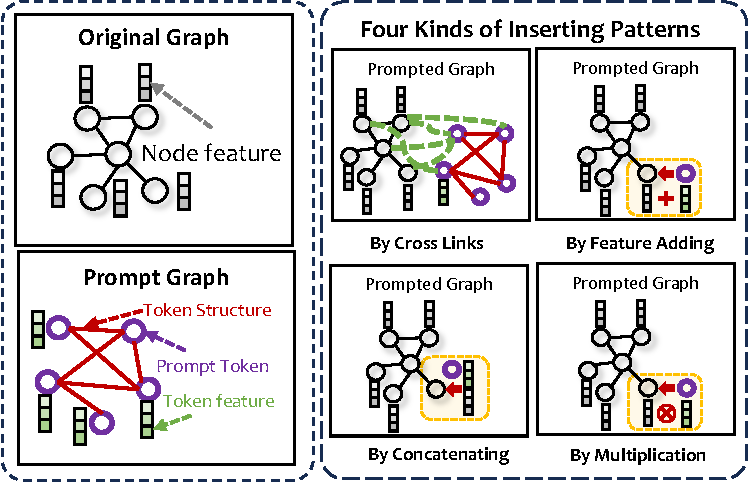
\includegraphics[width=0.49\textwidth]{pic/prompt.pdf}
    \caption{提示token、token结构与插入模式。}
    \label{fig:prompt}
\end{figure}



\subsection{提示token、结构与插入模式}\label{subsec:pdesign}

\textit{\dotuline{问题1：他们如何设计图提示？}}

\textbf{A. 将提示视为token。}
最简单的图提示可以被看作是向原始图特征中加入额外特征\cite{zhu2023graphcontrol}。例如，给定图特征矩阵
$\mathbf{X}=\{x_1,\cdots, x_N\} \in \mathbb{R}^{N\times d}$，
其中 $x_i\in \mathbb{R}^{1\times d}$ 为第 $i$ 个节点特征，$d$ 为特征空间维度。
\citet{fang2022prompt} 与 \citet{shirkavand2023deep} 将基础提示定义为一个可学习向量 $p \in \mathbb{R}^{1\times d}$，并将其加到所有节点特征上，使得被操控后的特征矩阵为
$\mathbf{X}^{*}=\{x_1+p,\cdots, x_N+p\}$。
通过这种方式，可使用重表述后的特征替代原始特征，并用预训练图模型处理该图。后续工作\cite{fang2023universal}进一步将单个提示token扩展为多个token，从而提升性能。PGCL\cite{gong2023prompt}为语义视角设计一个提示向量、为上下文视角设计另一个提示向量，并通过逐元素乘法将它们作用于图级表示；VNT\cite{tan2023virtual}同样采用类似的提示设计，但其插入模式并非将提示token加到原始节点特征上，而是将提示token与原始节点集合进行拼接，并借助图Transformer的自注意力机制完成融合。

在GraphPrompt\cite{liu2023graphprompt}中，提示token与\citet{fang2022prompt}定义的形式类似，但其差异在于：此前工作通常在输入特征空间中设计提示token，而GraphPrompt假设提示位于图模型的隐藏层空间。由于隐藏层维度通常小于原始输入特征维度，其提示token也相对更“短”。另一个差异是：该图提示用于辅助图池化（graph pooling）操作（即$\text{Readout}$）。例如，给定节点集合 $\mathcal{V}=\{v_1,\cdots, v_{|\mathcal{V}|}\}$，节点 $v$ 的嵌入为 $\textbf{h}_v \in \mathbb{R}^{1\times d}$，针对任务 $t$ 的提示token为 $\textbf{p}_t \in \mathbb{R}^{1\times d}$，则通过逐元素乘法（$\otimes$）将提示插入后得到：
$\textbf{s}_t=\text{Readout}(\{\textbf{p}_t \otimes \textbf{h}_v:v \in \mathcal{V}\})$。
类似地，SGL-PT\cite{zhu2023sglpt}创建一个提示token并将其连接到图中所有节点；该token具备全局感知能力，可辅助其预训练任务中的全局分支（也可视作一种池化策略）。

为对齐节点分类与链接预测，GPPT\cite{sun2022gppt}将图提示定义为额外token，包含任务token与结构token：其中任务token描述待分类的下游节点标签，结构token表征目标节点周围子图。通过这种方式，可将“预测节点 $v$ 的标签”重表述为“预测 $v$ 的结构token与标签任务token之间的潜在链接”。面向节点分类任务，ULTRA-DP\cite{chen2023ultradp}为每个目标节点创建一个提示token，其特征为目标节点的位置嵌入与预训练任务嵌入的加权和。HetGPT\cite{ma2023hetgpt}设计包含节点token与类别token的提示组织方式，与GPPT相似；不同之处在于其还加入类型特定的特征token，使提示对不同节点类型敏感，从而可扩展到异构图场景。



\textbf{B. 将提示视为图。}
All in One\cite{sun2023all}中的图提示是一张可通过高效调参学习得到的额外子图。提示token对应一些新增节点，其表示维度与原始节点表示一致。作者假设提示token与原始节点特征处于同一语义空间，从而便于用这些token操控原始节点特征。token结构包含两部分：一是不同提示token之间的内部连接；二是提示子图与原始图之间的跨连接。这些连接可通过token之间（内部连接）或token与原始节点之间（跨连接）的点积相似度进行预计算。插入模式则是：通过跨连接将提示子图并入原始图，将组合后的图视作新图输入，并送入预训练图模型得到图级表示。

PRODIGY\cite{huang2023prodigy}的提示图由数据图与任务图构成。数据图可以是目标节点周围子图（用于节点分类）、节点对（用于边分类），或直接为图分类实例；在这一部分，提示token与结构与原始图一致。任务图包含数据token与标签token：每个数据token连接到一个数据图，并进一步与标签token相连。不同于通过“提示下游数据”将下游任务重表述为预训练任务的思路，PRODIGY利用提示图来统一上游与下游任务；其预训练策略包含邻居匹配与标签匹配等任务，可重表述为预测提示图中数据token与标签token之间的相似性。SAP\cite{ge2023enhancing}同样将若干提示token（每个token对应一个类别）按All in One定义的跨连接方式连到原始图上；不同之处在于，其提示任务为节点级对比任务：用MLP编码节点特征形成第一视图，用GNN编码“加入提示后的图”形成第二视图，与其预训练任务保持一致。



\subsection{通过回答函数实现任务对齐}\label{subsec:align}

\textit{\dotuline{问题2：他们如何将下游任务重表述为预任务？}}

\textbf{A. 处理不同层级的任务。}
All in One\cite{sun2023all}通过图级对比学习进行预训练，其目标是在由原图扰动得到的多种图视图之间学习鲁棒图编码器。为将多类图任务对齐到该图级预任务，作者首先通过诱导子图将节点级、边级与图级任务统一到图级任务（这一思路也出现在PRODIGY\cite{huang2023prodigy}、GraphPrompt\cite{liu2023graphprompt}与PGCL\cite{gong2023prompt}中）。随后他们提出：向原图加入图提示本质上可视作对各种图操作（如节点特征掩码、节点/边扰动、子图移除等）的模拟。因此，只需为下游图数据集加入合适的图提示，就有望进一步将下游任务重表述为预任务。

\textbf{B. 可学习的回答函数。}
为了输出下游任务结果，\citet{sun2023all}设计了两类回答函数。第一类是可学习任务头（例如MLP映射），可在极少数据下进行调参。它以预训练图模型输出的图级表示为输入，并输出下游预测结果。例如，下游是三分类的节点分类任务，则可用包含三个输出单元的全连接层连接图表示（该图表示由预训练模型在“节点包含的组合图+图提示”上产生）。此时图提示与任务头均可调参，可交替更新。类似的可学习回答函数也在\cite{fang2022prompt, fang2023universal,tan2023virtual}等工作中采用。其优点是对齐任务较为直接，但也会增加调参流程的复杂度。

\textbf{C. 手工构造的回答函数。}
为进一步降低调参开销，All in One\cite{sun2023all}还提出第二类回答函数：不引入可训练任务头，而是手工构造推断规则。例如，对于节点分类，可设置 $K$ 个互异的子提示，每个子提示对应一个节点类别，$K$为类别总数。若预训练任务类似GraphCL\cite{you2020graph}，即最大化图级视图对的相似性，则当第$\ell$个提示图与原始“节点包含图”最相似时，可将目标节点预测为标签$\ell$（$\ell=1,2,\cdots,K$）。类似地，GPPT\cite{sun2022gppt}与HetGPT\cite{ma2023hetgpt}将链接预测作为预训练任务，并通过统一的任务模板将下游节点分类重表述为同一任务形式：将节点标签视作额外token后，可用预训练模型直接输出“标签token与目标节点之间存在边”的概率。

SAP\cite{ge2023enhancing}的预训练策略是比较来自两种图视图的节点表示：第一视图由节点特征编码得到，第二视图由图模型编码得到。为此，其提示token表示类别信息，并通过比较节点表示与各类别token的相似度，选取最大者作为预测类别。通过统一任务模板，PRODIGY\cite{huang2023prodigy}利用手工构造的提示图，将节点、边与图分类任务统一为“预测数据token与标签token之间的链接”。\citet{liu2023graphprompt}将链接预测扩展为图对相似度任务并作为预训练目标；为对齐下游节点分类与图分类任务，作者设计统一回答模板使下游端与预训练端对齐。具体而言，给定诱导图三元组 $(g_1,g_2, g_3)$，其中 $g_1$与$g_2$同类、$g_1$与$g_3$异类（当目标任务为节点分类时，诱导图对应目标节点上下文子图），统一回答模板定义为：$\text{sim}(g_1,g_2)>\text{sim}(g_1,g_3)$。



\subsection{提示调参（Prompt Tuning）}\label{subsec:pt}

\textit{\dotuline{问题3：他们如何学习图提示？}}

\textbf{A. 元学习技术。}
为学习合适的提示，\citet{sun2023all}采用元学习技术（如MAML\cite{finn2017modelagnostic}）以获得提示参数的鲁棒初始化点。由于支持集与查询集涵盖多种图任务（节点分类、链接预测、图分类等），学习到的图提示被期望在多类下游任务上具有更强的通用性。

\textbf{B. 任务特定调参。}
除All in One\cite{sun2023all}旨在学习跨任务通用提示外，也有工作针对特定下游任务（如图分类）进行更具任务指向性的提示调参。例如，GPF\cite{fang2022prompt}面向图分类任务，仅需通过最大化在提示图表示 $\tilde{\textbf{s}}_i$ 上预测正确标签的似然，联合调参提示token $\textbf{p}$ 与任务头 $\phi$。其目标可写为：
$\max_{\textbf{p}, \phi} \sum_{(y_i,\tilde{\textbf{s}}_i)} p_{\pi, \phi} (y_i| \tilde{\textbf{s}}_i)$，
其中 $\pi$ 表示预训练模型参数。

\textbf{C. 与预任务一致的调参。}
直观上，提示的目标是将下游任务重表述为预训练任务，因此若提示调参目标与预训练预任务一致，将更为自然。GraphPrompt\cite{liu2023graphprompt}建议使用与预训练相似的损失来学习提示。类似地，GPPT\cite{sun2022gppt}与VNT\cite{tan2023virtual}分别采用与其预训练任务（链接预测）与下游任务（节点分类）一致的交叉熵损失。HetGPT\cite{ma2023hetgpt}与SAP\cite{ge2023enhancing}采用节点级对比损失来学习提示token，因为其预训练也使用同类对比任务。PGCL\cite{gong2023prompt}引入图级损失以与预训练任务对齐。ULTRA-DP\cite{chen2023ultradp}提出两个预训练任务（边预测与邻居预测），每个任务对应一个任务嵌入；预训练时随机选择一个任务并将相应任务嵌入注入提示token，并与图模型共同训练。这些可学习任务嵌入随后可用于初始化下游提示。



\subsection{进一步讨论}\label{subsec:pdiscussion}

\textit{\dotuline{问题4：它们的联系、优缺点是什么？}}

GPF\cite{fang2022prompt}的优势在于其提示形式非常简单，可方便地复用于多种预训练与下游任务；但将单一提示token加到所有节点上在表达能力与泛化性方面较为受限。一个潜在改进是为每个节点学习独立提示token（即“一节点一提示”），但这会带来较高的参数开销。为此，GPF-Plus\cite{fang2023universal}训练 $K$ 个相互独立的基向量，并用它们组合生成各节点token，从而在参数效率与表达能力之间取得更好的平衡，这也使其思想更接近All in One\cite{sun2023all}。

HetGPT\cite{ma2023hetgpt}将提示token扩展为类型特定格式，可处理异构图中的图提示问题，但其下游主要针对节点分类。为扩展到更广任务范围，GraphPrompt\cite{liu2023graphprompt}将链接预测重表述为图对相似度任务。值得注意的是，其提示token的角色与图注意力网络中的投影向量较为相似；也存在一些基于注意力的图池化方法与其动机相近。差异在于：作者指出预训练阶段的图池化组件可能无法适配其他下游任务，因此需要额外提示来“重定向”图模型中的池化组件。

GPPT\cite{sun2022gppt}可被视作All in One\cite{sun2023all}更一般框架中的一个特例。例如，若将提示图简化为与节点类别相关的孤立token，并将生成图替换为完全图，则All in One的提示结构可退化为GPPT格式，从而使边级预任务可用于下游节点分类。GPPT的不足在于其预任务受限于二元边预测，且在下游主要对节点分类有效。相比之下，GraphPrompt与All in One旨在适配更广泛的图任务，不仅限于节点级分类。另一方面，当适配不同任务时，GraphPrompt、GPF与GPF-Plus往往需要额外调参一个任务特定模块；而All in One与GPPT更多依赖任务模板，强调对输入数据的操控，较少依赖下游任务的特定形式。

直观上，PRODIGY\cite{huang2023prodigy}中的数据图与All in One与GraphPrompt中的诱导图较为相似；其预训练任务可视为预测数据token与标签token之间的链接，与GPPT的思想也较为接近。其优点在于提示无可训练参数，因此无需调参，适合上下文学习（in-context learning）场景，也可用于不同数据集间的知识迁移。然而，不可调的提示通常不够灵活，在下游任务所在领域与预训练领域差异较大时可能限制泛化。相对地，ULTRA-DP\cite{chen2023ultradp}在预训练与下游阶段均进行提示调参：其先在预训练阶段学习任务嵌入（作为提示的核心组成之一），再用这些任务嵌入初始化下游提示。其提示并非用于将下游任务重表述为预任务，而更像是在任务池中选择更适配下游任务的预训练目标。如何在效率、泛化与灵活性之间取得最优平衡，仍是值得进一步研究的问题。

与多数工作显式定义插入模式不同，VNT\cite{tan2023virtual}将提示token与原始节点集合拼接后整体输入图Transformer。图Transformer通过自注意力机制计算它们之间的相关性，可视作All in One定义的插入模式的一个变体。其优点是无需人为设定阈值来裁剪连接；但局限在于其骨干必须是图Transformer，难以直接迁移到基于消息传递的图模型。此外，一些更先进的图Transformer变体需要额外的位置编码作为输入；而VNT中的提示token未显式与原图建立插入连接，使得将现有位置编码方法自然扩展到该场景并不容易。



\section{多模态与多领域中的图提示}\label{subsec:pmodal}

\subsection{含图的多模态提示}\label{subsec:multi_modal}

图像、声音与文本等多模态融合已被广泛研究并取得显著成功。然而，这些模态多由线性数据结构描述。在真实世界中，仍存在大量以图等非线性结构呈现的数据。如何将线性模态（如文本、图像、声音等）与非线性模态（如图）连接起来，已成为极具吸引力的研究主题，因为这代表着迈向人工通用智能的重要一步。不幸的是，实现这一愿景十分困难。目前，我们仅看到在文本与图的融合，尤其是带文本属性的图（text-attributed graphs）上取得了相对“硬核”的进展。随着大语言模型的发展，文本与图的融合变得更为容易，并取得更显著的性能提升。鉴于该主题已有较为系统的综述，我们在此仅简要讨论与\textit{\dotuline{提示技术}}密切相关的代表性工作；更多细节可参考\cite{li2023survey,liu2023graph}。

\textbf{A. 带文本属性图中的提示。}
\citet{wen2023augmenting}提出Graph-Grounded Pre-training and Prompting（G2P2），用于在数据资源受限时增强文本分类。其指出监督学习中标注数据不足的问题，并利用文本数据的网络结构（如超链接或引文网络）作为额外信息源。G2P2在预训练阶段采用文本-图交互策略并结合对比学习，在分类阶段引入新颖的提示机制，从而在零样本与少样本文本分类中表现出良好效果。\citet{zhao2023gimlet}面向分子性质预测这一标注稀缺领域，提出融合图与文本的模型，以增强零样本的基于提示的分子任务学习；该模型使用广义位置嵌入，并将图编码与任务提示解耦，从而提升跨新任务的泛化能力。\citet{li2023promptbased}在多模态（文本与图）节点分类的有限标注场景下进行研究：不同于传统将预计算文本特征喂给GNN的方法，他们通过手工语言提示模板在模型设计层面同时引入原始文本与图拓扑结构。

\textbf{B. 大语言模型在图数据处理中的作用。}
\citet{chen2023exploring}研究了大语言模型（LLMs）在图节点分类任务中的潜力，并提出两类流程：LLMs-as-Enhancers（用LLM增强节点文本属性，再由GNN预测）与LLMs-as-Predictors（直接用LLM作为预测器）。其实验表明，深句向量模型与基于LLM的文本增强能够有效提升节点属性质量；同时LLM作为独立预测器也有一定潜力，但在准确性与测试数据泄漏方面存在风险。\citet{fatemi2023talk}系统研究了将图结构数据编码为可供LLM消费的形式，并指出图编码方式、任务类型与图结构特性都会显著影响LLM性能；其结果显示简单提示对基础图任务更有效，且图编码函数对推理能力影响显著。\citet{jin2023patton}提出PATTON框架，在富含文本的网络上预训练语言模型，强调文本属性与网络结构的协同：其设计两种新预训练策略，一种在网络上下文中进行掩码语言建模，另一种预测被掩码节点，从而捕捉文本与网络结构的交互；在文档分类、检索与链接预测等任务上验证了优越性。\citet{wang2023knowledge}提出Knowledge Graph Prompting（KGP）用于多文档问答（MD-QA）：其先构建跨文档知识图，节点表示段落或文档结构，边表示语义/词法相似性；LM引导的图遍历器在图中收集支撑段落以辅助LLM回答问题，实验表明知识图构建与遍历器设计会显著影响性能。

\textbf{C. 基于图与提示的多模态融合。}
近年来，利用图结构与提示技术进行多模态融合取得了显著进展。例如，\citet{edwards2023synergpt}在药物协同预测中提出SynerGPT，采用Transformer结构，将上下文学习与遗传算法结合以预测药物协同效应。在视觉-语言模型领域，\citet{li2023graphadapter}提出GraphAdapter，采用基于提示的adapter式调参机制，通过双知识图将文本与视觉模态连接起来。\citet{liu2023gitmol}提出GIT-Mol，将多模态融合拓展到分子科学：大语言模型在提示的帮助下同时整合图、图像与文本数据，在分子生成与性质预测等任务上获得显著提升。尽管过去几年已投入大量努力，学界仍在探索更优方案，以通过带文本属性图或知识图实现文本与图的高效融合；同时，在更多模态融合方面仍存在广阔的想象空间与研究机会。



\subsection{基于提示的图领域自适应}\label{subsec:pdomain}
图领域自适应近年来取得了显著进展，提示技术的引入进一步推动了该方向发展。但总体而言，图领域自适应仍未被彻底解决，至少存在两项核心挑战：其一是不同领域间语义空间如何对齐；其二是结构差异如何识别与弥合。

\textbf{A. 语义对齐。}
All in One\cite{sun2023all}通过引入多任务提示与统一提示格式，将“预训练-微调”工作流扩展为“预训练-提示”，并以元学习优化提示参数。为提升图模型对不同图领域的适应性，作者首先指出图提示本质上可视作图操作，并据此用图提示对不同领域的图数据进行操控。GraphControl\cite{zhu2023graphcontrol}借鉴ControlNet提出部署模块，将下游特定信息作为条件输入引入，从而提升预训练模型对目标数据的适应性；该方法在不同图之间对齐输入空间，并注入目标数据的特有性质。\citet{zhang2023structure}提出用于知识图迁移学习的预训练模型，并采用通用提示调参机制：将任务数据视作三元组提示，使任务KG与任务数据能灵活交互。\citet{yi2023contrastive}将个性化图提示与对比学习结合，用于跨领域推荐，尤其适用于冷启动场景。\citet{liu2023one}提出代表性方法：用语言描述不同领域的图节点，再用LLM得到文本嵌入以实现对齐；但该方法依赖每个特征具有可解释的语义名称，而在许多场景中图特征往往是缺乏明确语义的潜在向量。

\textbf{B. 结构对齐。}
\citet{cao2023when}分析不同图数据集间的可迁移性，并指出结构差异会对各类图模型可迁移性形成上界约束。GraphGLOW\cite{zhao2023graphglow}旨在突破闭世界假设（测试图与训练图相同），指出对每个图数据集从头训练结构学习模型会带来高昂计算成本与过拟合风险。为此，GraphGLOW将一个跨图共享的结构学习器与多个图特定的GNN协同训练，以捕捉跨数据集可泛化的最优消息传递拓扑模式；结构学习器训练完成后，可在无微调的情况下为未见目标图生成自适应结构，从而显著降低训练时间与资源。AAGOD\cite{guo2023datacentric}提出面向GNN的OOD检测数据中心框架，其使用参数化放大矩阵（可视为提示）叠加到输入图的邻接矩阵上。\citet{shirkavand2023deep}受提示调参启发提出DeepGPT用于图Transformer：在输入图与每个Transformer层均加入提示token，并通过更新这些提示token实现对不同图数据集的高效调参。
